% --------------------------------------------------------------
% This is all preamble stuff that you don't have to worry about.
% Head down to where it says "Start here"
% --------------------------------------------------------------
 
\documentclass[12pt]{article}
 
\usepackage[margin=1in]{geometry} 
\usepackage{amsmath,amsthm,amssymb,scrextend}
\usepackage{fancyhdr}
\usepackage{enumitem}
\usepackage{amsmath}
\usepackage{amssymb}
\usepackage{textcomp}
\usepackage{fancybox}
\usepackage{tikz}
\usepackage{tasks}
\pagestyle{fancy}
\usepackage[makeroom]{cancel}
\usepackage{graphicx}
\usepackage{caption}
\usepackage{mwe}
\usepackage{tikz}
\usetikzlibrary{positioning}

\newcommand{\N}{\mathbb{N}}
\newcommand{\Z}{\mathbb{Z}}
\newcommand{\I}{\mathbb{I}}
\newcommand{\R}{\mathbb{R}}
\newcommand{\Q}{\mathbb{Q}}
\renewcommand{\qed}{\hfill$\blacksquare$}
\let\newproof\proof
\renewenvironment{proof}{\begin{addmargin}[1em]{0em}\begin{newproof}}{\end{newproof}\end{addmargin}\qed}
% \newcommand{\expl}[1]{\text{\hfill[#1]}$}
 
\newenvironment{theorem}[2][Theorem]{\begin{trivlist}
\item[\hskip \labelsep {\bfseries #1}\hskip \labelsep {\bfseries #2.}]}{\end{trivlist}}
\newenvironment{lemma}[2][Lemma]{\begin{trivlist}
\item[\hskip \labelsep {\bfseries #1}\hskip \labelsep {\bfseries #2.}]}{\end{trivlist}}
\newenvironment{problem}[2][Problem]{\begin{trivlist}
\item[\hskip \labelsep {\bfseries #1}\hskip \labelsep {\bfseries #2.}]}{\end{trivlist}}
\newenvironment{exercise}[2][Exercise]{\begin{trivlist}
\item[\hskip \labelsep {\bfseries #1}\hskip \labelsep {\bfseries #2.}]}{\end{trivlist}}
\newenvironment{reflection}[2][Reflection]{\begin{trivlist}
\item[\hskip \labelsep {\bfseries #1}\hskip \labelsep {\bfseries #2.}]}{\end{trivlist}}
\newenvironment{proposition}[2][Proposition]{\begin{trivlist}
\item[\hskip \labelsep {\bfseries #1}\hskip \labelsep {\bfseries #2.}]}{\end{trivlist}}
\newenvironment{corollary}[2][Corollary]{\begin{trivlist}
\item[\hskip \labelsep {\bfseries #1}\hskip \labelsep {\bfseries #2.}]}{\end{trivlist}}
 
\setlength{\parindent}{0pt}
\begin{document}
 \settasks{
	counter-format=(tsk[r]),
	label-width=4ex
}
% --------------------------------------------------------------
%                         Start here
% --------------------------------------------------------------

\lhead{Math 632}
\chead{Homework 4}
\rhead{Meenmo Kang}

\noindent
\textbf{Problem 1}\\
Consider these two Markov chains given in terms of their transition graphs (the first one has state space $\{a,b,c,d\}$ and the second one state space $\{a,b,c\}$).
$$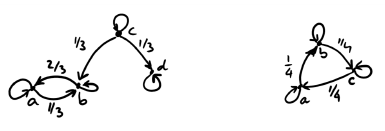
\includegraphics[height=4cm, width=12cm]{hw4_1.png}$$
Address the following questions for each of the two Markov chains
\begin{enumerate}[label=(\alph*)]
    \item Find all invariant distributions that satisfy detailed balance.
    $$
    \begin{pmatrix}
    \pi_1&\pi_2&\pi_3&\pi_4
    \end{pmatrix}
    \cdot
    \begin{pmatrix}
    2/3&1/3&0&0\\
    2/3&1/3&0&0\\
    0&1/3&1/3&1/3\\
    0&0&0&1
    \end{pmatrix}
    $$
    
\begin{align*}
    \pi_a &= \frac{2}{3}\pi_a + \frac{2}{3}\pi_b     & \qquad\qquad
    \pi_b &= \frac{1}{3}\pi_a + \frac{1}{3}\pi_b + \frac{1}{3}\pi_c\\
    \pi_c &= \frac{1}{3}\pi_c    &   
    \pi_d &= \frac{1}{3}\pi_c+\pi_d
\end{align*}

So we obtain, $$\pi_a = 2\pi_b \qquad \pi_c=0 \qquad\pi_d=1-3\pi_b$$
Thus the invariant matrix is
$$\pi=
\begin{pmatrix}
2\pi_b&\pi_b&0&1-3\pi_b
\end{pmatrix}$$

Let's check if it satisfies the detailed balance.
$$\pi_c\; p(c,d) = \pi_d\; p(d,c)\quad \Leftrightarrow\quad 0\cdot \frac{1}{3} = (1-3\pi_b)\cdot 0$$
$$\pi_a\; p(a,b) = \pi_b\; p(b,a)\quad \Leftrightarrow\quad 2\pi_b\cdot \frac{1}{3} = \pi_b\cdot \frac{2}{3}$$

\vspace{1.5\baselineskip}
Therefore we can observe that it holds the detailed balance.

\newpage
    \item Does the Markov chain have invariant distributions that do not satisfy detailed balance? Explain.
    $$
    \begin{pmatrix}
    \pi_1&\pi_2&\pi_3
    \end{pmatrix}
    \cdot
    \begin{pmatrix}
    3/4&1/4&0\\0&3/4&1/4\\1/4&0&3/4
    \end{pmatrix}$$

So we obtain,
\begin{align*}
    \pi_a &= \frac{3}{4}\pi_a + \frac{1}{4}\pi_c     & \qquad
    \pi_b &= \frac{1}{4}\pi_a + \frac{3}{4}\pi_b     & \qquad
    \pi_c &= \frac{1}{4}\pi_c + \frac{3}{4}\pi_c \\
\end{align*}
$$\Leftrightarrow \pi_a=\pi_b=\pi_c \qquad
\text{ i.e. } \pi = \begin{pmatrix} 1/3&1/3&1/3 \end{pmatrix}$$
   
\vspace{1.5\baselineskip}
Then let's check if it satisfies the detailed balance. 

$$\pi_a\;(a,b) = \frac{1}{3}\cdot \frac{1}{4} \neq \pi_b\;(b,a) = \frac{1}{3}\cdot 0$$

\vspace{1.5\baselineskip}
Therefore, it does not satisfy the detailed balance.
\end{enumerate}


\newpage
\textbf{Problem 2}\\
A Markov chain has four states $\{a,b,c,d\}$. Once the chain is in state d it stays there. From $a$ or $b$ the process jumps to one of the other three states with equal probability. From $c$ the process jumps to a or $b$ with equal probability.\\
Compute $E_a[T_d],\; E_b[T_d],$ and $E_c[T_d]$.
$$P=
\begin{pmatrix}
0&1/3&1/3&1/3\\
1/3&0&1/3&1/3\\
1/2&1/2&0&0\\
0&0&0&1
\end{pmatrix}$$

\vspace{1.5\baselineskip}

\begin{itemize}
    \item $E_a[T_d] = 1 + \frac{1}{3}E_b[T_d] + \frac{1}{3}E_c[T_d]$
    \item $E_b[T_d] = 1 + \frac{1}{3}E_a[T_d] + \frac{1}{3}E_c[T_d]$
    \item $E_c[T_d] = 1 + \frac{1}{2}E_a[T_d] + \frac{1}{2}E_b[T_d]$\\
    
    \item $E_a[T_d] = 1 + \frac{1}{3}E_b[T_d] + \frac{1}{3}\left(1 + \frac{1}{2}E_a[T_d] + \frac{1}{2}E_b[T_d]\right)
    =\frac{4}{3} + \frac{1}{6}E_a[T_d] +\frac{1}{2}E_b[T_d]
    $
    \item $\frac{5}{6}E_a[T_d] = \frac{1}{2}E_b[T_d] + \frac{4}{3}$
    \item $E_a[T_d] =  \frac{3}{5}E_b[T_d] + \frac{8}{5}$\\
    
    \item  $E_b[T_d] = 1 + \frac{1}{3}\left(\frac{3}{5}E_b[T_d] + \frac{8}{5}
    \right)
    + \frac{1}{3}\left(1 + \frac{1}{2}E_a[T_d] + \frac{1}{2}E_b[T_d] \right)$
    
    \item $E_b[T_d] = \frac{28}{15}+\frac{1}{6}E_a[T_d] +\frac{11}{30}E_b[T_d]    $
    \item $\frac{19}{30}E_b[T_d] = \frac{28}{15}+\frac{1}{6}E_a[T_d]$
    \item $E_b[T_d] = \frac{56}{19}+\frac{5}{19}E_a[T_d]$\\
    
    \item $E_b[T_d] = \frac{56}{19}+\frac{5}{19}\left(\frac{3}{5}E_b[T_d] + \frac{8}{5}
    \right)$
    \item $\frac{16}{19}E_b[T_d] = \frac{64}{19} \;\; \Leftrightarrow \;\; E_b[T_d] = 4$\\
    
    \item $E_a[T_d] =  \frac{3}{5}\cdot 4 + \frac{8}{5} = 4$
    \item $E_a[T_d] = 5$
\end{itemize}





\newpage
\textbf{Problem 3}\\
Consider the following graph: the vertices are the points
$$S = \{(i,j)\;|\;i,j\in \{1,2,3,4\}\}$$
Two vertices $(i, j)$ and $(i',j')$ are connected if either $i=i',\; j=j' \pm 1,$ or $j=j'$ and $i=i'\pm 1$.\\
$$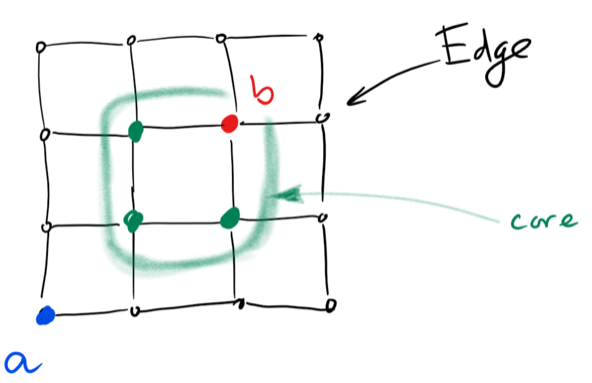
\includegraphics[height=4cm, width=7cm]{hw4_3.png}$$
The core of the graph is $C = \{(i,j)\;|\;i,j\in\{2,3\}\}$. The edge of the graph consists of all points that are not in the core. Let $X_n$ be the Markov process that describes a random walk on $S$. Define $T=min\{n\ge 0\;|\; X_n\in C\}.$\\
Explain how you can compute the probability $P[X_T = b\;|\;X_0 = a]$ where $a =(1,1)$ and $b=(3,3)$. You should provide enough detail so that someone with a computer or calculator could use your explanation to compute $P[X_T=b\;|\;X_0 = a]$.

\vspace{2\baselineskip}
There are four cases

\begin{tasks}(4)
\task edge$\to$edge
\task edge$\to$core
\task core$\to$core
\task core$\to$edge
\end{tasks}

\vspace{1.5\baselineskip}
\begin{enumerate}
    \item Construct 16 x 16 transition matrix.
    \item Consider another transition matrix for $P(edge,core)$
    $$p(edge,core)=
    \begin{pmatrix}
    &(2,2)&(2,3)&(3,2)&(3,3)\\
    (1,1)&0&0&0&0\\
    (1,2)&1/3&0&0&0\\
    \vdots&\ldots&\ldots&\ldots\\
    (4,3)&0&0&0&1/3\\
    (4,4)&0&0&0&0
    \end{pmatrix}    $$
    
    \item Calculate $\left(I-P_{edge,edge}\right)^{-1}\cdot P_{edge,core}$
    \item Remind that (1,1) is transient and (3,3) is recurrent.
\end{enumerate}


\newpage
\textbf{Exercise 1.56}\\
A bank classifies loans as paid in full (F), in good standing (G), in arrears
(A), or as a bad debt (B). Loans move between the categories according to the
following transition probability:

$$
\begin{matrix}
    &\textbf{F}&\textbf{G}&\textbf{A}&\textbf{B}\\
\textbf{F}&1&0&0&0\\
\textbf{G}&.1&.8&.1&0\\
\textbf{A}&.1&.4&.4&.1\\
\textbf{B}&0&0&0&1\\
\end{matrix}$$

\begin{enumerate}[label=(\alph*)]
\item What fraction of loans in good standing are eventually paid in full?
    \begin{itemize}
        \item Due to the property for the gambler's ruin, $P(T_F<\infty)$ should be found.
        
        \item $P_G(T_F<\infty) = 0.1 + 0.8\times P_G(T_F<\infty) + 0.1\times P_A(T_F<\infty)$\\
        $\Rightarrow 0.2\times P_G(T_F<\infty) = 0.1 + 0.1\times P_A(T_F<\infty)$\\
        $\Rightarrow P_G(T_F<\infty) = \frac{1}{2} + \frac{1}{2}\times P_A(T_F<\infty)$
        \vspace{1.5\baselineskip}
        
        \item $P_A(T_F<\infty) = 0.1 + 0.4\times P_G(T_F<\infty) + 0.4\times P_A(T_F<\infty)$\\
        $\Rightarrow 0.6\times P_A(T_F<\infty) = 0.1 + 0.4\times P_G(T_F<\infty)$\\
        $\Rightarrow P_A(T_F<\infty) = \frac{1}{6} + \frac{4}{6}\times P_G(T_F<\infty)$
        \vspace{1.5\baselineskip}
        
        \item $P_G(T_F<\infty) = \frac{1}{2} + \frac{1}{2} \times \left(\frac{1}{6} + \frac{4}{6}\times P_G(T_F<\infty)\right) =\frac{1}{2} + \frac{1}{12}+ \frac{1}{3}P_G(T_F<\infty)$\\ 
        $\Rightarrow \frac{2}{3} P_G(T_F<\infty) = \frac{7}{12}$\\
        $\Rightarrow P_G(T_F<\infty) = \frac{7}{8}$
        \vspace{1.5\baselineskip}
        
    \end{itemize}


\item What is the answer for those in arrears?
    
    $$P_A(T_F<\infty) = \frac{1}{6} + \frac{4}{6}\times P_G(T_F<\infty) = \frac{1}{6} + \frac{2}{3}\times \frac{7}{8} = \frac{3}{4}$$
    
\end{enumerate}

















\newpage
\textbf{Exercise 1.58}\\
Six children (Dick, Helen, Joni, Mark, Sam, and Tony) play catch. If Dick has the ball he is equally likely to throw it to Helen, Mark, Sam, and Tony. If Helen has the ball she is equally likely to throw it to Dick, Joni, Sam, and Tony. If Sam has the ball he is equally likely to throw it to Dick, Helen, Mark, and Tony. If either Joni or Tony gets the ball, they keep throwing it to each other. If Mark gets the ball he runs away with it. 

\begin{enumerate}[label=(\alph*)]
    \item Find the transition probability and classify the states of the chain.
    
\begin{minipage}[t]{0.4\textwidth}
          \centering\raisebox{\dimexpr \topskip-\height}{
          $P=
            \begin{pmatrix}
            &\textbf{D}&\textbf{S}&\textbf{H}&\textbf{T}&\textbf{J}&\textbf{M}\\
            \textbf{D}&0&1/4&1/4&1/4&0&1/4\\
            \textbf{S}&1/4&0&1/4&1/4&0&1/4\\
            \textbf{H}&1/4&1/4&0&1/4&1/4&0\\
            \textbf{T}&0&0&0&0&1&0\\
            \textbf{J}&0&0&0&1&0&0\\
            \textbf{M}&0&0&0&0&0&1
            \end{pmatrix}$
            \quad
            
            
            }
        \end{minipage}\hfill
        \begin{minipage}[t]{0.4\textwidth}
          \centering\raisebox{\dimexpr \topskip-\height}{
            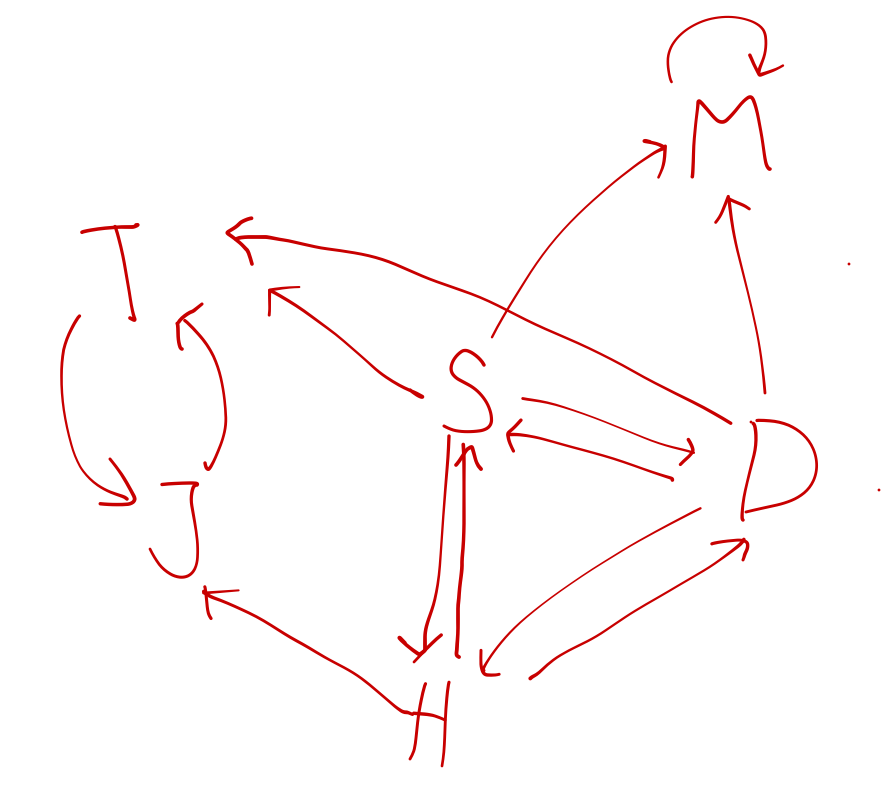
\includegraphics[height=4cm, width=4cm]{hw4_2.png}
        }
        \end{minipage}
%    $$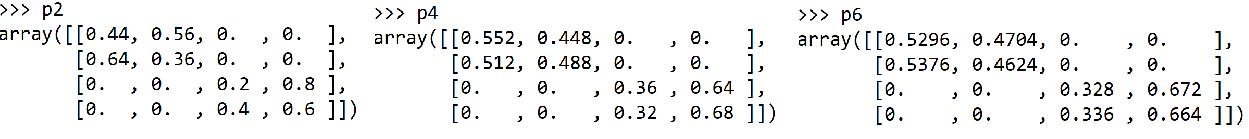
\includegraphics[width=\textwidth]{hw3_np1.png}$$


    \item Suppose Dick has the ball at the beginning of the game. What is the probability Mark will end up with it?
    \begin{itemize}
        \item Note that once it enters to either T, J, there is no probability that the ball is thrown to Mark at the end.
    
        \item $P_D(T_M<\infty) = \frac{1}{4}P_S(T_M<\infty) + \frac{1}{4}P_H(T_M<\infty) + \frac{1}{4}$
        
        \item $P_S(T_M<\infty) = \frac{1}{4}P_D(T_M<\infty) + \frac{1}{4}P_H(T_M<\infty) + \frac{1}{4}$
        
        \item $P_H(T_M<\infty) = \frac{1}{4}P_D(T_M<\infty) + \frac{1}{4}P_S(T_M<\infty)$\\

        \item $P_D(T_M<\infty) = \frac{1}{4}P_S(T_M<\infty) + \left(\frac{1}{16}P_D(T_M<\infty) + \frac{1}{16}P_S(T_M<\infty)\right) + \frac{1}{4}$
        
        \item $\frac{15}{16} P_D(T_M<\infty) = \frac{5}{16}P_S(T_M<\infty) + \frac{1}{4}$
        
        \item $P_D(T_M<\infty) = \frac{1}{3}P_S(T_M<\infty) + \frac{4}{15}$\\
        
        \item $P_S(T_M<\infty) = \frac{1}{4}P_D(T_M<\infty) + \frac{1}{4}\left(\frac{1}{4}P_D(T_M<\infty) + \frac{1}{4}P_S(T_M<\infty)\right) + \frac{1}{4}$
        
        \item $\frac{15}{16}P_S(T_M<\infty) = \frac{5}{16}P_D(T_M<\infty) +  \frac{1}{4} $
        
        \item $P_S(T_M<\infty) = \frac{1}{3}P_D(T_M<\infty) +  \frac{4}{15}$\\
        
        \item $P_D(T_M<\infty) = \frac{1}{3}\left(\frac{1}{3}P_D(T_M<\infty) +                                            \frac{4}{15}\right) + \frac{4}{15}$
        \item $\frac{8}{9} P_D(T_M<\infty) = \frac{16}{45}$
        \item $P_D(T_M<\infty) = \frac{16}{45}\cdot \frac{9}{8} = \mathbf{\frac{2}{5}}$
\end{itemize}
    
\end{enumerate}







\newpage
\textbf{Exercise 1.67}\\
Roll a fair die repeatedly and let $Y_1,Y_2,...$ be the resulting numbers. Let $X_n=|\{Y_1,Y_2,...,Y_n\}|$ be the number of values we have seen in the first $n$ rolls for $n\ge 1$ and set $X_0=0$. $X_n$ is a Markov chain. 
\begin{enumerate}[label=(\alph*)]
    \item Find its transition probability.\\
    
    \begin{minipage}[t]{0.4\textwidth}
              \centering\raisebox{\dimexpr \topskip-\height}{%
              \begin{pmatrix}
                0&1&0&0&0&0&0\\
                0&1/6&5/6&0&0&0&0\\
                0&0&2/6&4/6&0&0&0\\
                0&0&0&3/6&3/6&0&0\\
                0&0&0&0&4/6&2/6&0\\
                0&0&0&0&0&5/6&1/6\\
                0&0&0&0&0&0&1
              \end{pmatrix}
            }
            
            \end{minipage} \hfill
            \begin{minipage}[t]{0.65\textwidth}
              \vspace{1.5\baselineskip}
              \qquad\;\;
              \begin{cases}
              
                    $P(x_{n+1} = i\;|\;x_n=i) = \frac{i}{6}$\\
                    $P(X_{n+1} = i+1\;|\;x_n=i) = \frac{6-i}{6}$
              \end{cases}
            \end{minipage}
    
    \vspace{3\baselineskip}
    
    \item Let $T = min\{n: X_n = 6\}$ be the number of trials we need to see all 6 numbers at least once. Find ET.\\
    
    $$(I-P_{TT}) = \begin{pmatrix}
    1&-1&0&0&0&0\\
    0&5/6&-5/6&0&0&0\\
    0&0&4/6&-4/6&0&0\\
    0&0&0&3/6&-3/6&0\\
    0&0&0&0&2/6&-2/6\\
    0&0&0&0&0&1/6
    \end{pmatrix}$$
    
    $$
    (I-P_{TT})^{-1} = \begin{pmatrix}
    1&6/5&3/2&2&3&6\\
    0&6/5&3/2&2&3&6\\
    0&0&3/2&2&3&6\\
    0&0&0&2&3&6\\
    0&0&0&0&3&6\\
    0&0&0&0&0&6
    \end{pmatrix}
    $$
    
    $$
    \vec{m} = (I-P_{TT})^{-1}\cdot \begin{pmatrix}
    1&1&1&1&1&1
    \end{pmatrix}^T
    =
    \begin{pmatrix}
    1&6/5&3/2&2&3&6\\
    0&6/5&3/2&2&3&6\\
    0&0&3/2&2&3&6\\
    0&0&0&2&3&6\\
    0&0&0&0&3&6\\
    0&0&0&0&0&6
    \end{pmatrix}
    \cdot
    \begin{pmatrix}
    1\\1\\1\\1\\1\\1
    \end{pmatrix}
    $$
    
    \vspace{1.5\baselineskip}
    $$ET = 1+\frac{6}{5}+\frac{3}{2}+2+3+6=14.7$$
\end{enumerate}

\end{document}